\documentclass[landscape]{tikzposter}
% tikzposter automatically loads tikz, graphicx 

\usetheme{Wave} % Rays, Basic, Simple, Envelope, Wave, Board, Autumn, Desert
\usecolorstyle{Spain} % Default, Australia, Britain, Sweden, Spain, Russia, Denmark, Germany
\usebackgroundstyle{Rays} % Default, Rays, VerticalGradation, BottomVerticalGradation, Empty 
\usetitlestyle{Wave} % Default, Basic, Envelope, Wave, VerticalShading, Filled, Empty
\useblockstyle{Basic} % Default, Basic, Minimal, Envelope, Corner, Slide, TornOut
\tikzposterlatexaffectionproofoff % Removes logo in bottom right corner
% See the tikzposter manual for more custom colors and styles

\usepackage{mathptmx}
\usepackage{bookman}

\usepackage{amsmath,amssymb}

\usepackage[
  pdftitle = {Cal Poly Math 351}, 
  pdfauthor = {Tony Mendes}, 
  pdfsubject = {Typesetting}, 
  colorlinks = true, 
  urlcolor = blue, 
  linkcolor = blue, 
  citecolor = blue]{hyperref}

\title{\textup{\textbf{Conference Posters}}} %\textup disables the default small caps in title
\author{Tony Mendes}
\institute{Cal Poly San Luis Obispo}

\begin{document}

\maketitle 

\begin{columns}

\column{0.66}

\block{How to use the Tikzposter class}{
\vspace{1ex}
\begin{itemize}
\item Use \texttt{tikzposter} in \texttt{documentclass}, not \texttt{article}. \\[1ex]
\item Create columns using \\[1ex] 
\texttt{\textbackslash begin\{columns\}  \\
\textbackslash \{column\}\{X\} \\
... \\
\textbackslash \{column\}\{Y\} \\
... \\
\textbackslash \{column\}\{Z\} \\
... \\
\textbackslash begin\{columns\} } \\[1ex]
where $\texttt{X, Y}$ and $\texttt{Z}$ are percentages which sum to $1$.  They control the column 
widths. \\[1ex]
\item Create blocks within columns using \texttt{\textbackslash block\{title\}\{content\}}. \\[1ex]
\item Read the manual at  
\href{https://www.ctan.org/pkg/tikzposter}{\texttt{www.ctan.org/pkg/tikzposter}}
for more information. \\[2ex]
\end{itemize}
}
\note[width = 13cm, angle = 10, radius = 30cm, rotate = -15]{
Everyone loves puppies!  
\begin{center}

\includegraphics[height = 5in]{puppy}
\end{center}
}

\column{0.33}

\block{Common poster mistakes}{
\begin{itemize}
\item Too much content! \\[1ex]
\item Lots of text and mathematics and/or a cramped design. \\[1ex]
\item No images of cute puppies. \\[1ex]
\item Warning: \texttt{theorem}, \texttt{proof}, \texttt{verbatim} cannot be used.
\end{itemize}
}

\block{A puppy}{
\begin{center}
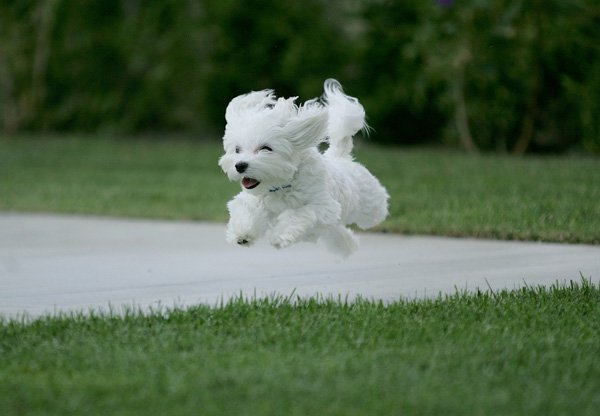
\includegraphics[width = 7.5in]{puppy2.jpg}
\end{center}
}


\end{columns}

\begin{columns}
\column{0.5}
\block{The Fundamental Theorem of Algebra}{

\textbf{Theorem.} Every polynomial $f(x) = a_n x^n + \cdots + a_0$ has a root 
in $\mathbb{C}$. \\[2ex]

\innerblock{A sktech of a proof}{

  When $r \approx 0$, we see \( f(r e^{i \theta}) \approx a_0 \).  \\[2ex]
  
  When $r$ is big, we see $f(r e^{i \theta}) \approx a_n r^n e^{i n \theta}$.  
  These are $n$ giant circles in the complex plane.  \\[2ex]

  So as $r$ changes from $0$ to $\infty$, there are values $r, \theta$ which make
  $f(r e^{i \theta})$ cross the origin in the complex plane. \\[2ex]
}
}

\column{0.5}

\block{An example when $f(x) = x^3 - x + 1$}{
  
  \begin{center}

  $f(r e^{i \theta})$ for $\theta \in [0,2 \pi)$ shown on the complex plane: \\[2ex]
  
  \begin{tikzpicture}[scale = 2.5]
    \node at (0,-3) {$r = .1$};
    \draw [->, thin] (-1.5,0) -- (2.5,0);
    \draw [->, thin] (0,-2) -- (0,2);
    \draw (1, .05) -- (1, -.05) node [below] {$1$};
    \draw [domain=0:2*pi, samples = 100, smooth, ultra thick, blue]
      plot ({1 - 0.1*cos(\x r) + 0.001*cos(3*\x r)}, {-0.1*sin(\x r) + 0.001*sin(3*\x r)});
  \end{tikzpicture}
  \hspace{5ex}
  \begin{tikzpicture}[scale = 2.5]
    \node at (0,-3) {$r = .5$}; 
    \draw [->, thin] (-1.5,0) -- (2.5,0);
    \draw [->, thin] (0,-2) -- (0,2);
    \draw (1, .05) -- (1, -.05) node [below] {$1$};
    \draw [domain=0:2*pi, samples = 100, smooth, ultra thick, blue]
      plot ({1 - 0.5*cos(\x r) + 0.125*cos(3*\x r)}, {-0.5*sin(\x r) + 0.125*sin(3*\x r)});
  \end{tikzpicture}
  \hspace{5ex}
  \begin{tikzpicture}[scale = 2.5]
    \node at (0,-3) {$r = .75$}; 
    \draw [->, thin] (-1.5,0) -- (2.5,0);
    \draw [->, thin] (0,-2) -- (0,2);
    \draw (1, .05) -- (1, -.05) node [below] {$1$};
    \draw [domain=0:2*pi, samples = 100, smooth, ultra thick, blue]
      plot ({1 - 0.75*cos(\x r) + 0.421875*cos(3*\x r)}, {-0.75*sin(\x r) + 0.421875*sin(3*\x r)});
  \end{tikzpicture}
  \hspace{5ex}
  \begin{tikzpicture}[scale = 2.5]
    \node at (0,-3) {$r \approx 0.868837\dots$}; 
    \draw [->, thin] (-1.5,0) -- (2.5,0);
    \draw [->, thin] (0,-2) -- (0,2);
    \draw (1, .05) -- (1, -.05) node [below] {$1$};
    \draw [domain=0:2*pi, samples = 100, smooth, ultra thick, blue]
    plot ({1 - 0.868837*cos(\x r) + 0.655866*cos(3*\x r)}, {-0.868837*sin(\x r) + 0.655866*sin(3*\x r)});
  \end{tikzpicture}

  \end{center}
}
\end{columns}

\end{document}
